%\subsection{Electron Reconstruction}
%\label{subsec:electron_reco}
The electron reconstruction in ATLAS uses a dynamic, topological cell clustering approach to improve energy measurements. The process identifies topo-clusters that correspond to electron showers in the calorimeter, followed by a track-cluster matching and a \textbf{Gaussian-Sum Filter (GSF)} refit (see \ref{subsec:gsf}) for precision. As shown in Figure~\ref{fig:gsf-emcal-electron_reco}, the reconstruction proceeds through multiple stages, including matching conversion vertices for photons and adding satellite clusters to account for Bremsstrahlung photons emitted by electrons, improving energy resolution. The final electron object (as stored in the \verb|xAOD::Electron| container) consist of a cluster built from energy deposits in the EM calorimeter (supercluster) and a matched track (or more precisely xAOD::TrackParticle). While for an \verb|xAOD::Muon| object the linked \verb|xAOD::TrackParticle| is an ID track (InDetTrackParticles container), for an \verb|xAOD::Electron| it is a GSF \verb|xAOD::TrackParticle| (\verb|GSFTrackParticles| container). Note: each electron has a GSF track, but not every GSF track is linked to an electron. The ATLAS electron reconstruction is described in detail in~\cite{ATL-PHYS-PUB-2017-022}. 

\begin{figure}[!ht]
    \centering
    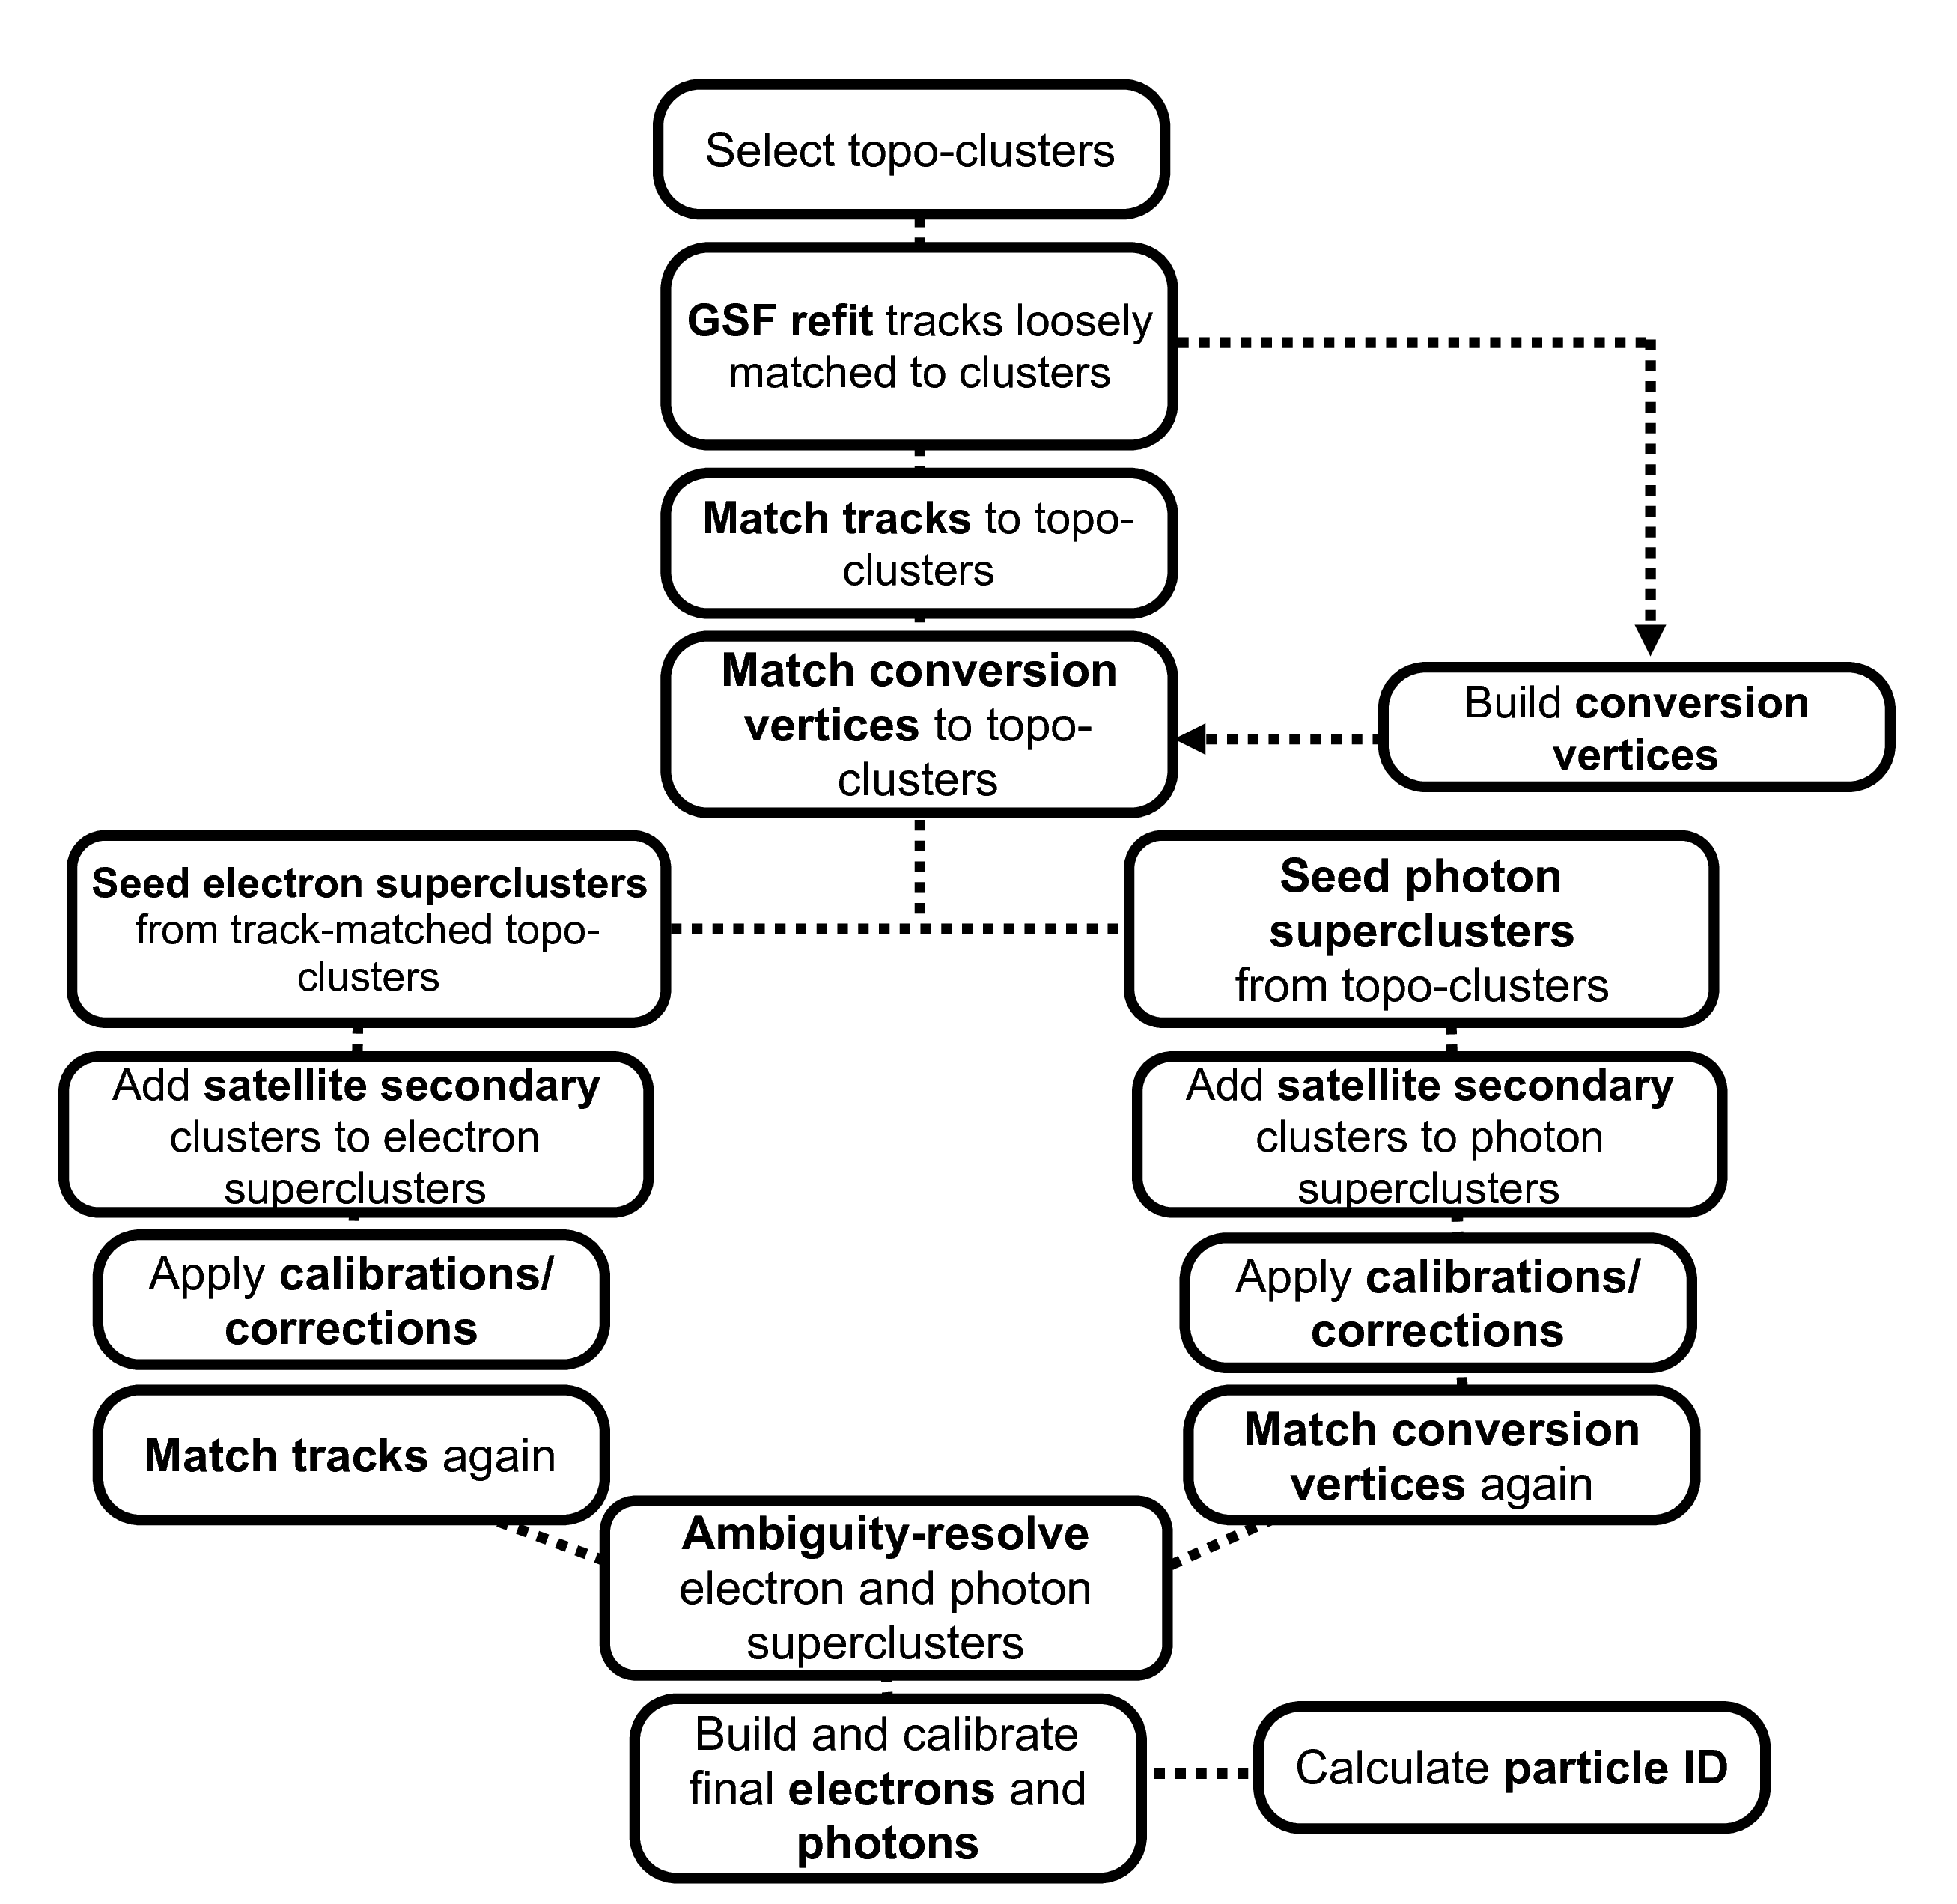
\includegraphics[width=0.7\textwidth]{figures/gsf_emcal_egamma_fig_02}
    \caption{Algorithm flow diagram for the new electron and photon reconstruction. Taken from~\cite{ATL-PHYS-PUB-2017-022}.}
    \label{fig:gsf-emcal-electron_reco}
\end{figure}


\subsubsection{Gaussian-Sum Filter Reconstruction}
\label{subsec:gsf}
Given the energy loss by electrons via Bremsstrahlung, the \textbf{Gaussian-Sum Filter (GSF)} reconstruction is employed to handle the non-Gaussian nature of the electron's energy loss. In contrast to standard Kalman filters used for most charged particles, which assume Gaussian errors, GSF accounts for the probabilistic energy loss by representing the electron track state as a weighted sum of multiple Gaussian components. This allows for a more accurate description of the particle's momentum at each step, improving the quality of the reconstructed track and enhancing the identification of electrons. However, a GSF \verb|xAOD::TrackParticle| is only a ``better'' ID \verb|xAOD::TrackParticle|, there is no EM calorimeter (EMCal) information involved in the fitting procedure.


\subsubsection{Problems with the Standard Electron Reconstruction}
To build our di-electron candidates a standard vertex fit is performed for all pairs of oppositely charged electrons passing the selection (in the event). Although the algorithm loops over the \verb|xAOD::Electron| container, more precise parameters of the linked GSF \verb|xAOD::TrackParticle| are actually used in the di-electron vertex fit. However, even this approach does not ensure an accurate reconstruction of the di-electron invariant mass. The $J/\psi \rightarrow e^+e^-$ peak is highly asymmetric because of the Bremsstrahlung losses and the candidates are leaking into the low-$q^2$ bin as shown in Figure~\ref{fig:gsf-emcal-m_jpsi_1}. As these low-$q^2$ $J/\psi$ candidates cannot be separated, they are also used in the $B$-meson candidate vertex fit, which leads to a huge irreducible background in the low-$q^2$ bin $B_d^0$ invariant mass distribution as shown in Figure~\ref{fig:gsf-emcal-m_bd_1}.

\begin{figure}[!ht]
    \centering
    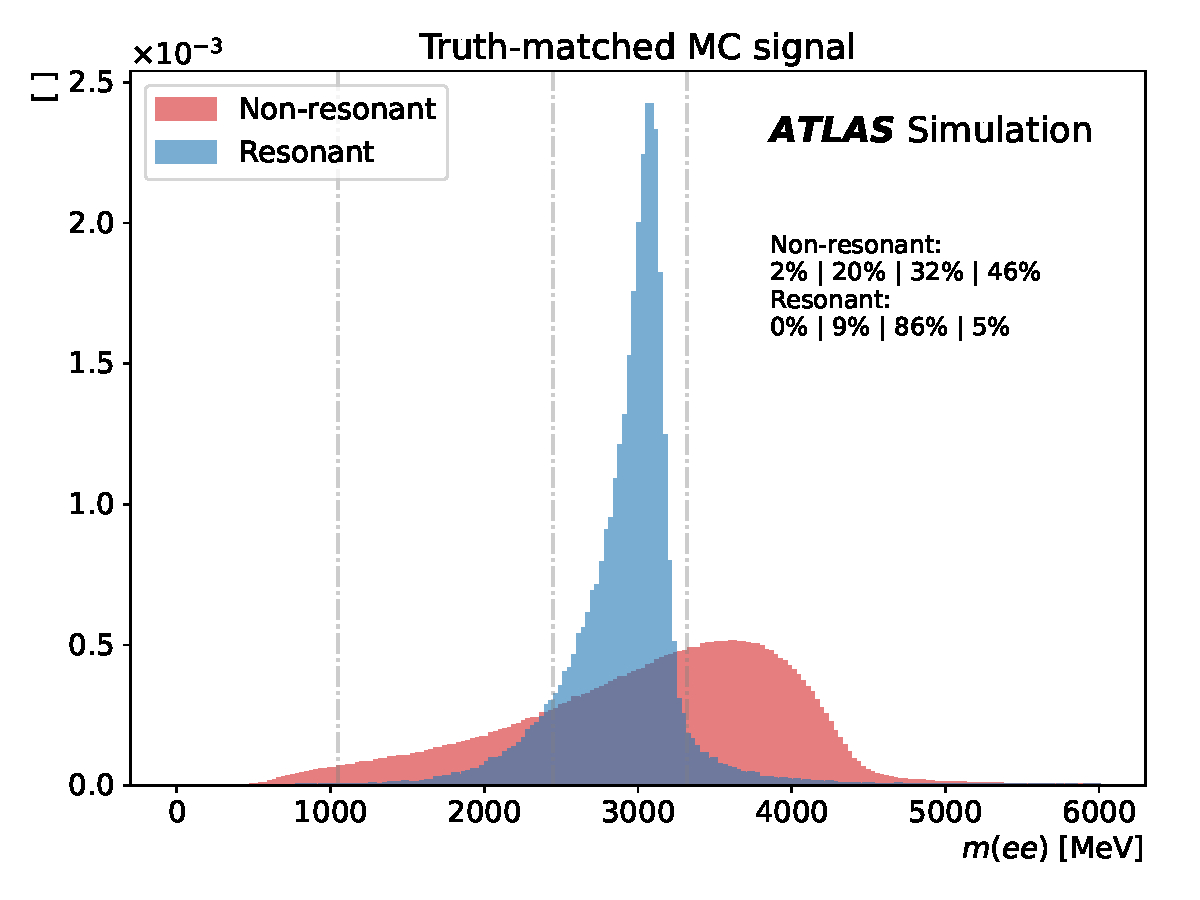
\includegraphics[width=0.7\textwidth]{figures/gsf_emcal_mee_q2full}
    \caption{Distribution of the di-electron invariant mass $m(e^+e^-)$ for the truth-matched $B_d^0 \rightarrow e^+e^- K^*$ (red) and $B_d^0 \rightarrow J/\psi(e^+e^-) K^*$ (blue) MC candidates. Dot-dashed lines indicate the boundaries of the low- and high-$q^2$ bins. Numbers shown in the figure show fraction of candidates in the below-low-$q^2$ bin, low-$q^2$ bin, high-$q^2$ bin and above-high-$q^2$ bin.}
    \label{fig:gsf-emcal-m_jpsi_1}
\end{figure}

\begin{figure}[!ht]
    \centering
    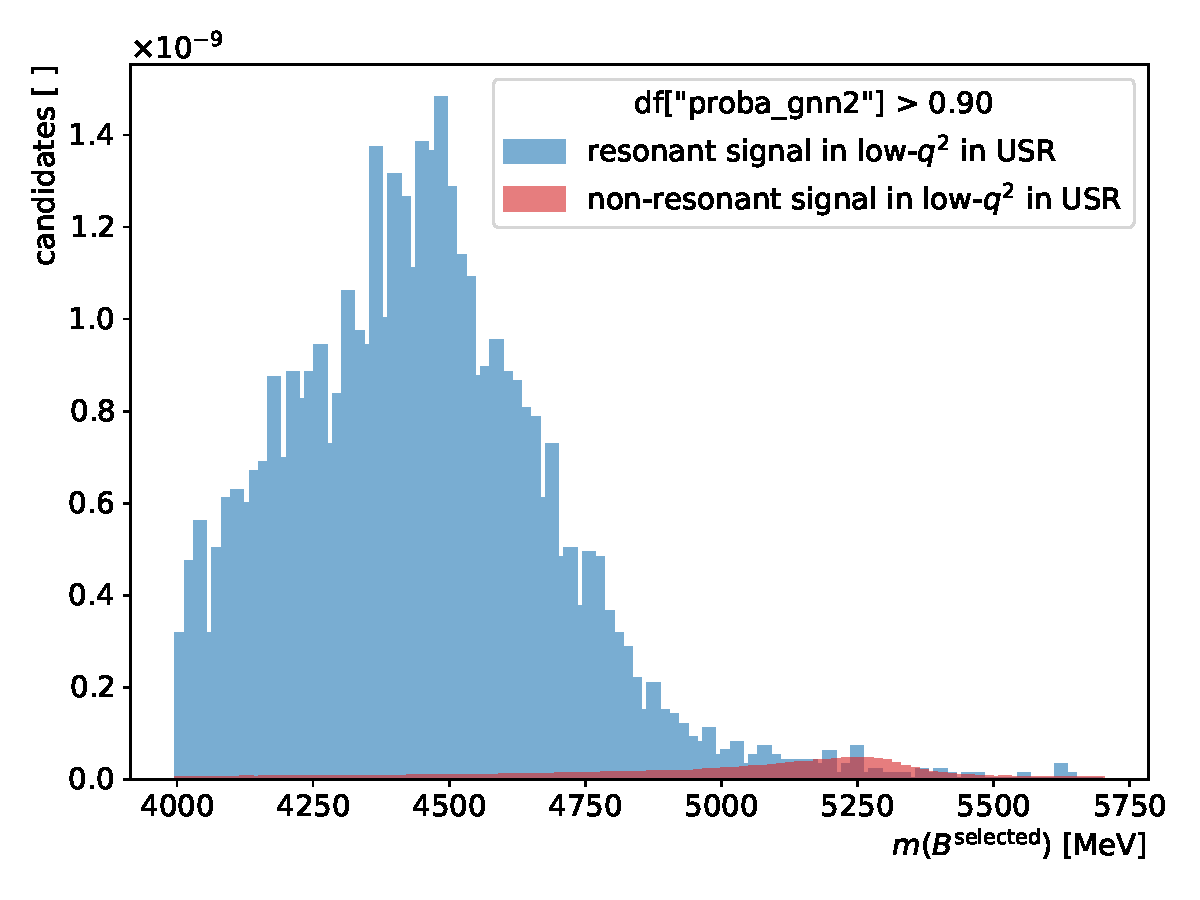
\includegraphics[width=0.7\textwidth]{figures/gsf_emcal_bd_mass_gnn2}
    \caption{Distribution of the invariant mass $m(B)$ for the truth-matched $B_d^0 \rightarrow e^+e^- K^*$ (red) and $B_d^0 \rightarrow J/\psi(e^+e^-) K^*$ (blue) MC candidates in the low-$q^2$ bin after the tight GNN2 selection ($P_\mathrm{GNN2} > 0.90$). Irreducible leaking resonant signal acts as a main background in the low-$q^2$ bin. [\textbf{\color{red}TODO:} Describe (or ``link'') GNN.]}
    \label{fig:gsf-emcal-m_bd_1}
\end{figure}


\subsection{Using EMCal Information in the Electron Track Fit}
To enhance our signal sensitivity in the low-$q^2$ bin, we need to either improve signal resolution, background rejection, or both. It turns out that both objectives can be achieved by incorporating the EMCal information into the (GSF) \verb|Trk::Track| fit, as illustrated in Figure~\ref{fig:gsf-emcal-gsf_emcal_idea}. A new detector ``hit'' is created using the supercluster coordinates, added to the original GSF track hits, and a new GSF fit is performed. Since most ATLAS analyses focus on high-$p_\mathrm{T}$ regions and low-$p_\mathrm{T}$ B-physics analyses typically use only muons, this approach had not been tested previously.

\begin{figure}[!ht]
    \centering
    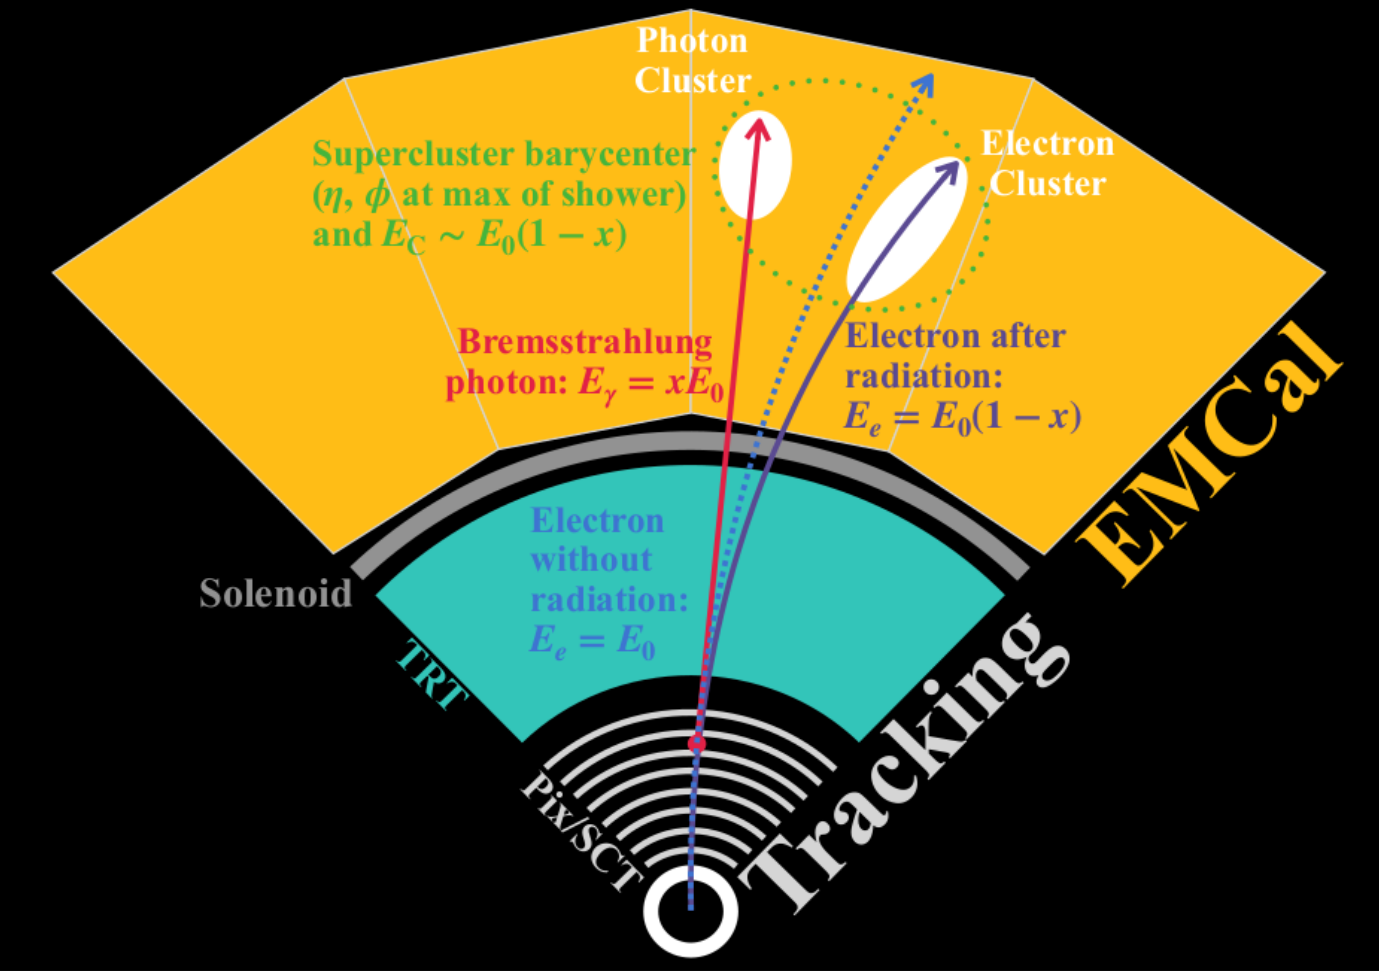
\includegraphics[width=0.7\textwidth]{figures/gsf_emcal_idea}
    \caption{General idea of using EMCal supercluster to improve the standard GSF reconstruction (fit).}
    \label{fig:gsf-emcal-gsf_emcal_idea}
\end{figure}


\subsubsection{Updated Workflow}
In the standard reconstruction, the GSF re-fit is performed during the ESD $\rightarrow$ AOD step. \verb|Trk::Track| objects, which contain individual hit information, are required, but the ``Track'' container is only retained in the ESD format. This format is created temporarily on-the-fly, while only the AOD format with \verb|xAOD::TrackParticle| is saved for further analysis. Di-electron and $B$-meson candidates vertex fits are performed in the AOD $\rightarrow$ DAOD step using \verb|xAOD::TrackParticle| exclusively. Fortunately, for \textbf{real data}, the \verb|Trk::Track| ``GSFTrack'' container is kept up to AOD, so no reprocessing from RAW is needed for an additional GSF re-fit. For MC samples, reprocessing from HITS is required to retain this container in the AOD. However, this is significantly less effort than modifying the standard ATLAS-wide reconstruction and reprocessing the real data.

The existing \verb|CaloCluster_OnTrackBuilder| was extended and, along with several other fixes and improvements, integrated into our \verb|BPHY| ``derivation'' framework. If requested, the new reconstruction process is initiated immediately prior to the di-electron vertex fitting sequence. It generates a new \verb|xAOD::TrackParticle| container containing the re-fitted tracks (further denoted as GSF+EMCal), which is subsequently used for the di-electron and $B$-meson vertex fits.

[\textbf{\color{red}TODO:} Link to the code and MR?]


\subsubsection{Comparison of Different Setups}
An EMCal-track-hit can be created using the energy ($E$), $\eta$, and $\phi$ coordinates (or any combination thereof) and corresponding uncertainties measured at various \textbf{depths} within the EMCal supercluster. Currently, only the ``entrance'' and ``middle'' depths are considered practical for use. Initial tests indicated [\textbf{\color{red}TODO:} Link to my presentation on the e/gamma meeting] that the energy variable is the primary factor driving the improvement, and therefore only combinations including this variable are considered.

Figure~\ref{fig:gsf-emcal-gsf_vs_gsf_emcal_mean_std} shows a comparison of the original and new electron track parameters for various reconstruction setups. The ``pre-vtx'' track parameters refer to those obtained from the GSF+EMCal re-fit, while the ``post-vtx'' parameters correspond to the same tracks after being fitted to a common vertex (the $B$-meson candidate vertex fit), which can change the curvature. The ``pre-vtx'' parameters reflect the direct improvements in the reconstruction, whereas the ``post-vtx'' parameters demonstrate the applicability of these improvements within the analysis. A clear improvement is observed in the reconstruction of electron $p_\mathrm{T}$ and the di-electron invariant mass. Other parameters show no significant improvement, with the standard deviation of the ``RECO-TRUE'' distributions being larger. However, the new reconstruction does not introduce any bias into these parameters. There is no significant difference between the use of different combinations of EMCal parameters. However, using only the energy (end its uncertainty) measured at \textbf{depth} = ``middle'' appears to yield slightly better results with the currently available calibration. Therefore, this combination has been selected as the new default.

\begin{figure}[!ht]
    \centering
    
\includegraphics[height=0.8\textwidth, angle=90]{gsf_vs_gsf_emcal_v81}
    \caption{Comparison of various new reconstruction setups. The ``pre-vtx'' track parameters refer to those obtained from the GSF+EMCal re-fit, while the ``post-vtx'' parameters correspond to the same tracks after being fitted to a common vertex (the $B$-meson candidate vertex fit), which can change the curvature. The ``pre-vtx'' parameters reflect the direct improvements in the reconstruction, whereas the ``post-vtx'' parameters demonstrate the applicability of these improvements within the analysis.}
    \label{fig:gsf-emcal-gsf_vs_gsf_emcal_mean_std}
\end{figure}


\subsection{Default GSF vs. GSF+EMCal Comparison}
The main improvements are summarised in this section. The most significant is the reduction of ``leaking'' $J/\psi \rightarrow e^+e^-$ events, as shown in Figure~\ref{fig:gsf-emcal-gsf_vs_gsf_emcal_mee_mc_latest}. [\textbf{\color{red}TODO:} add numbers!] As a result, the irreducible $B_d^0 \rightarrow J/\psi(e^+e^-) K^*$ background is reduced by approximately 75\% in the low-$q^2$ bin, and the $B_d^0 \rightarrow e^+e^- K^*$ signal peak becomes narrower and about 10\% higher, as illustrated in Figure~\ref{fig:gsf-emcal-bd_mass_comparison}. Figures~\ref{fig:gsf-emcal-gsf_vs_gsf_emcal_mee_data_latest} and~\ref{fig:gsf-emcal-gsf_vs_gsf_emcal_mb_data_latest} demonstrate similar improvements in the invariant mass for candidates reconstructed in real data from the 2018 period M. Additional selection cuts are applied to $B_d^0 \rightarrow J/\psi(e^+e^-) K^*$ candidates to reduce combinatorial and mis-reconstructed backgrounds, without which the signal peak would not be visible.

[\textbf{\color{red}TODO:} plots of m(ee) in BB, BE and EE regions using the latest version.]

[\textbf{\color{red}TODO:} do the m(ee) fits to get some numbers (e.g. FWHM) for the latest version.]

\begin{figure}[!ht]
    \centering
    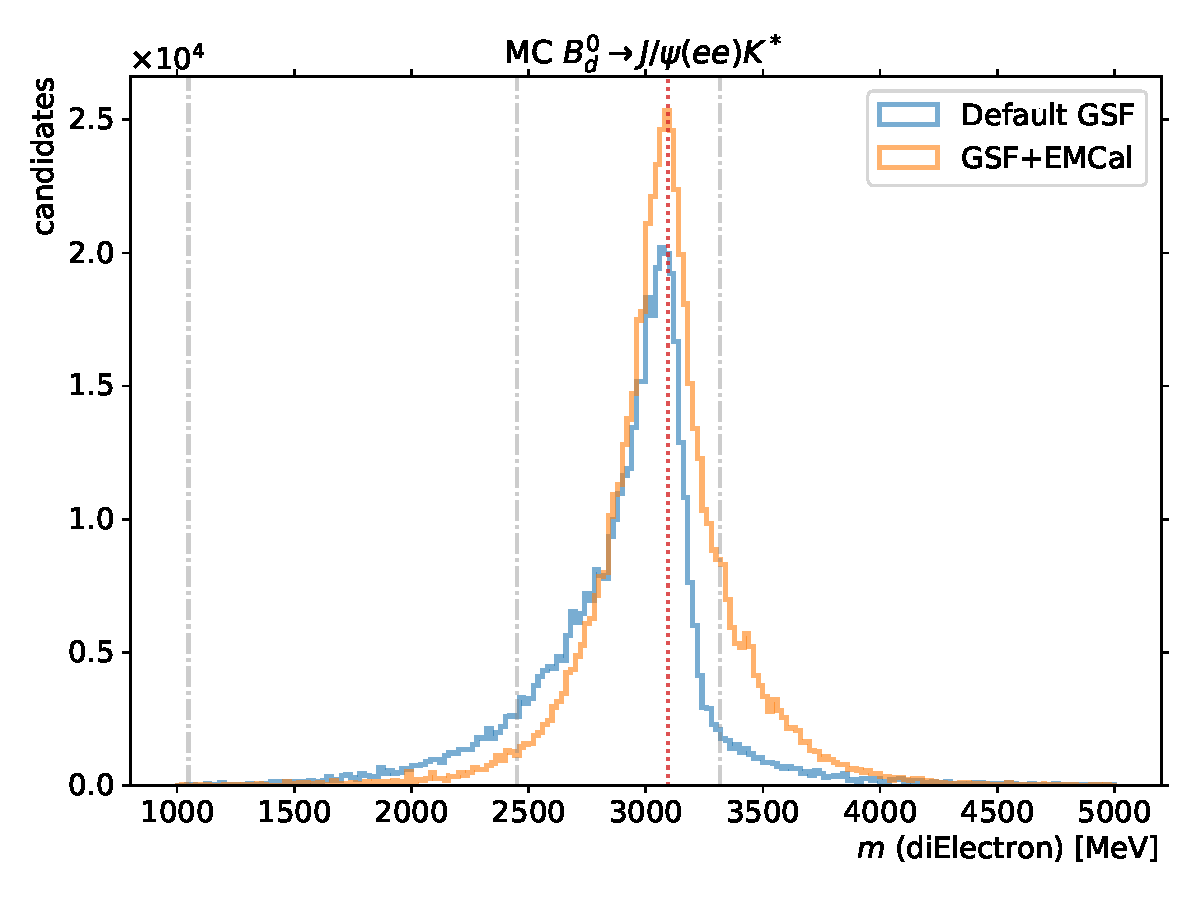
\includegraphics[width=0.7\textwidth]{figures/gsf_vs_gsf_emcal_mee_mc_latest}
    \caption{Distribution of the di-electron invariant mass for the truth-matched $B_d^0 \rightarrow J/\psi(e^+e^-) K^*$ MC candidates reconstructed using default GSF (blue) and GSF+EMCal (orange) methods. Dot-dashed lines indicate the boundaries of the low- and high-$q^2$ bins, while the red dotted line represents the current PDG value for the $J/\psi$ mass~\cite{ParticleDataGroup:2024cfk}.}
    \label{fig:gsf-emcal-gsf_vs_gsf_emcal_mee_mc_latest}
\end{figure}

\begin{figure}[!ht]
    \centering
    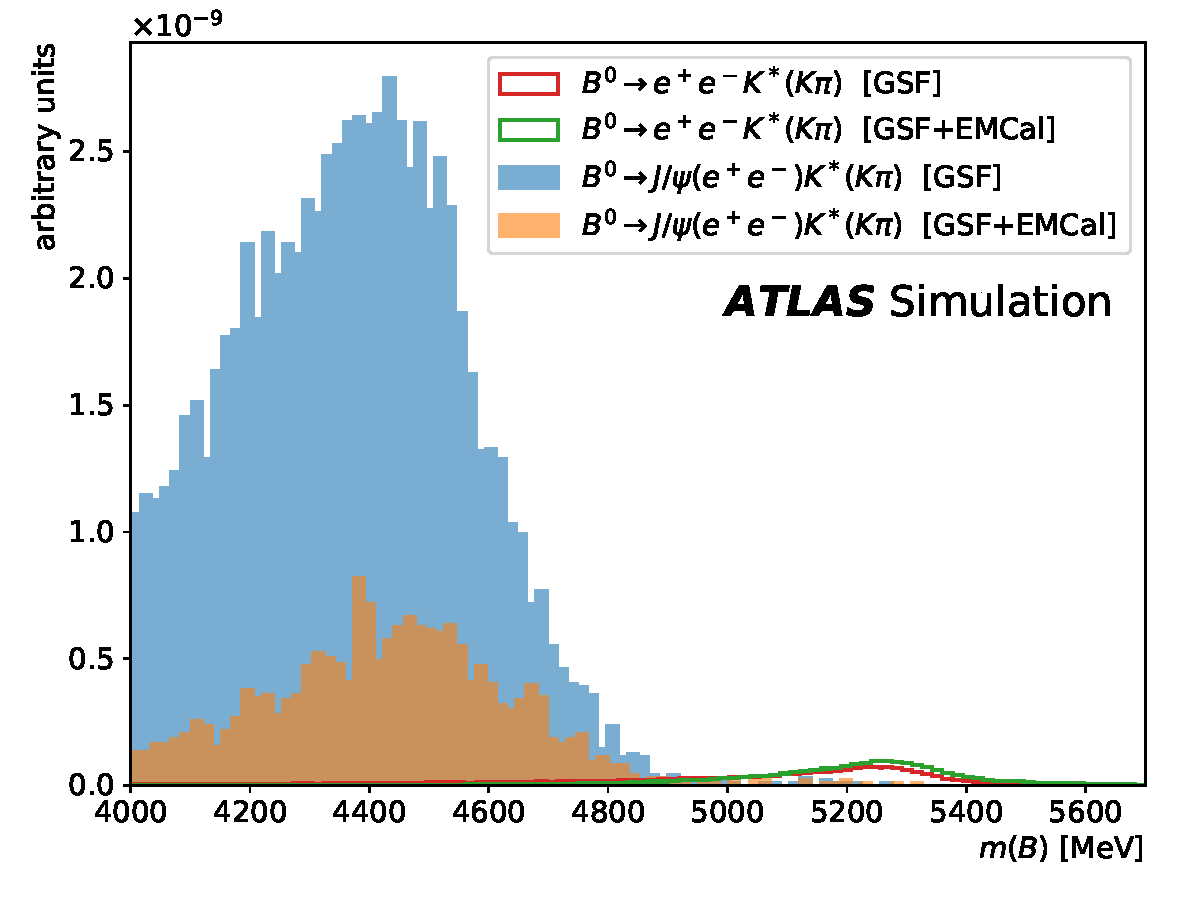
\includegraphics[width=0.7\textwidth]{figures/gsf_emcal_bd_mass_comparison}
    \caption{Distribution of the invariant mass $m(B)$ for the truth-matched $B_d^0 \rightarrow e^+e^- K^*$ (default GSF in red, GSF+EMCal in green) and ``leaking'' $B_d^0 \rightarrow J/\psi(e^+e^-) K^*$ (default GSF in blue, GSF+EMCal in orange) MC candidates in the low-$q^2$ bin. [\textbf{\color{red}TODO:} split the plot into ``default GSF'' and ``GSF+EMCal''?]}
    \label{fig:gsf-emcal-bd_mass_comparison}
\end{figure}

\begin{figure}[!ht]
    \centering
    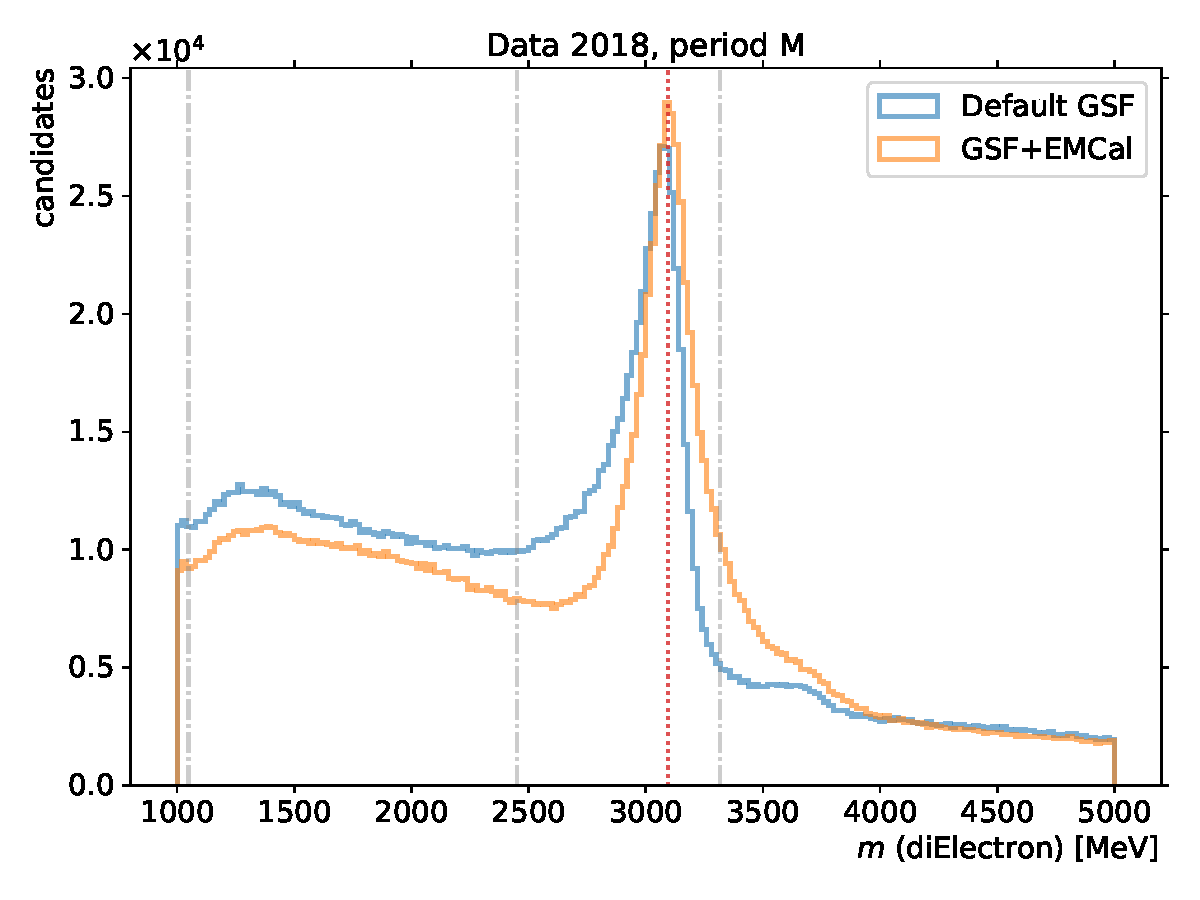
\includegraphics[width=0.7\textwidth]{figures/gsf_vs_gsf_emcal_mee_data_latest}
    \caption{Distribution of the di-electron invariant mass for the $B_d^0 \rightarrow J/\psi(e^+e^-) K^*$ candidates reconstructed in the real data (2018 period M) using default GSF (blue) and GSF+EMCal (orange) methods. Dot-dashed lines indicate the boundaries of the low- and high-$q^2$ bins, while the red dotted line represents the current PDG value for the $J/\psi$ mass~\cite{ParticleDataGroup:2024cfk}.}
    \label{fig:gsf-emcal-gsf_vs_gsf_emcal_mee_data_latest}
\end{figure}

\begin{figure}[!ht]
    \centering
    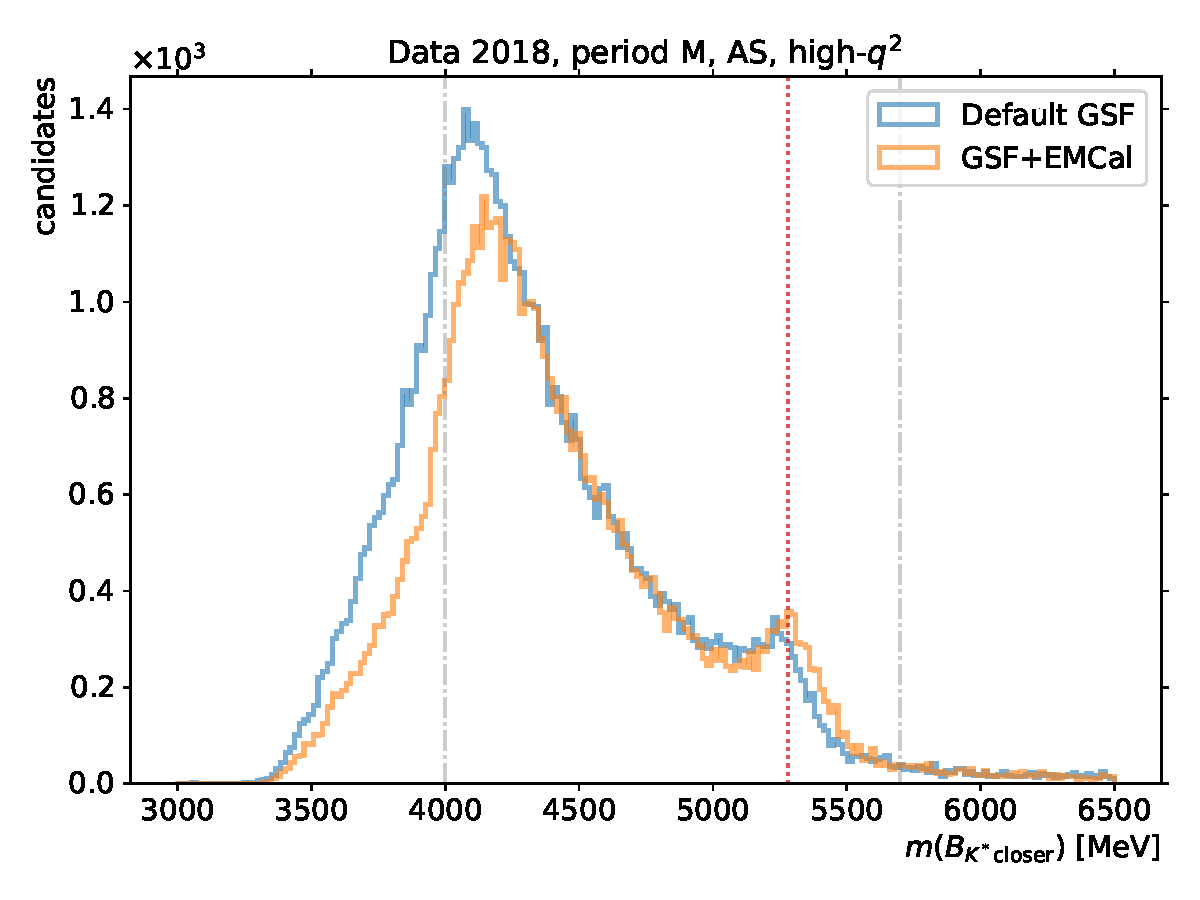
\includegraphics[width=0.7\textwidth]{figures/gsf_vs_gsf_emcal_mb_data_latest}
    \caption{Distribution of the invariant mass $m(B)$ for the $B_d^0 \rightarrow J/\psi(e^+e^-) K^*$ candidates reconstructed in the real data (2018 period M) using default GSF (blue) and GSF+EMCal (orange) methods. Dot-dashed lines indicate the boundaries of the signal region used in the final invariant mass fit, while the red dotted line represents the current PDG value for the $B_d^0$ mass~\cite{ParticleDataGroup:2024cfk}.}
    \label{fig:gsf-emcal-gsf_vs_gsf_emcal_mb_data_latest}
\end{figure}